\section{Real-Cluster Measurements}
\label{sec:real}

Simulation gives us control but assumes away the cost of knowing. We therefore ran the same
routing logic on real containers (\S\ref{sec:setup:real}): a single-node \texttt{k3s} cluster with
three worker pods, application-level link shaping, and a client outside the cluster. We report
three things the simulator cannot see, then the reproducibility of the comparison itself.

\subsection{The benefit needs network share, and tolerates little staleness}
At an offered load corresponding to $\rho_{\text{cpu}}=0.50$ and a 38.9 MB payload
(measured network share $0.65$), the network-aware policy beats the network-blind one in four of
four grid cells, by $21$--$45\%$ on p95. At a 0.6 MB payload (network share
$0.05$) the same comparison is $-1.6\%$, $+68.7\%$, $+23.1\%$, $-16.3\%$ --- i.e.~no effect or
harm. This is the same on/off behavior as \S\ref{sec:rq1}, on real kernel networking rather than
a model. Injecting a 3 s state lag reduces the benefit from $-45.2\%$ to $-21.4\%$ at
the moderate load and from $-37.5\%$ to $-27.9\%$ at the higher one, consistent with the
direction found in simulation.

\subsection{Reading state is not free, and gets slower exactly when it matters}
The simulator assumes an observation is instantaneous. On the cluster, fetching a worker's state
costs \SIrange{56}{876}{\milli\second} against 12 µs for an in-cluster network
round trip --- a factor of \numrange{50}{900}. More importantly, the cost is not constant: it
grows with system load, because the state endpoint competes for the same CPU quota as the work it
describes. This is a \emph{feedback loop} that simulation omits by construction: the busier the
system, the staler the observation, precisely when freshness matters most.

We also measured the floor that polling imposes. With a 15 s polling period, the
actual age of the state the scheduler acts on was 6.4 s on average and
14.8 s worst-case --- that is, roughly half a period to a full period, on top of any
export delay. A scheduler cannot be fresher than its polling loop, so ``zero lag'' is not
achievable in practice even when no network delay exists.

Two operational failure modes surfaced. First, the latency impact of stale state is
\emph{threshold-like}, not proportional: pulls taking 64 ms to
755 ms left p95 essentially unchanged, whereas pulls taking
3.6 s to 6.4 s made p95 \numrange{2}{3.6}$\times$ worse. In our setting
the knee sits between 1 s and 5 s. Second, when a state pull times out
(>2 s), our client substitutes a conservative ``everything is busy'' value, which
makes the scheduler effectively blind; this occurred twice in a long run and is a failure mode
worth designing for explicitly rather than discovering in production.

\subsection{How much can a single-node cluster claim?}
\begin{figure}[t]
\centering
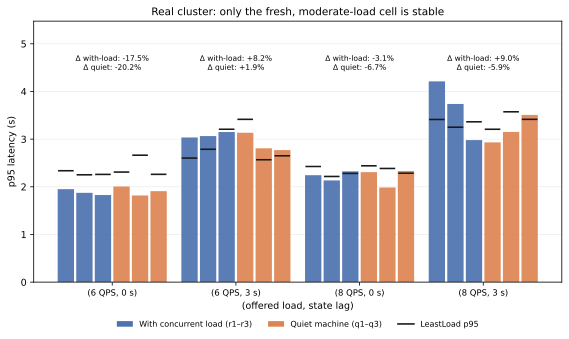
\includegraphics[width=\columnwidth]{figures/fig_real_cluster.svg}
\caption{Real cluster, six independent repeats per cell. Bars are the network-aware policy's p95
under three runs with a concurrent job on the host and three on an idle machine; short horizontal
marks are the network-blind baseline for the same run. Only the fresh, moderate-load cell has a
stable direction across all six.}
\label{fig:real}
\end{figure}
Because the earlier grid ran each cell once, we repeated a focused grid (two offered loads
$\times$ two staleness levels $\times$ the payload with $0.65$ network share) six times, three of
them while a simulation also ran on the same host and three on an otherwise idle machine.

\begin{table}[t]
\centering
\caption{Real cluster, six independent repeats of each cell ($\Delta$p95 of the network-aware
policy vs.\ the network-blind one; negative is better). Only the fresh, moderate-load cell has a
stable direction.}
\label{tab:realrepeats}
\footnotesize
\setlength{\tabcolsep}{4pt}
\begin{tabular}{@{}llrrrrrrr@{}}
\toprule
Load & State & \multicolumn{3}{c}{with a concurrent job} & \multicolumn{3}{c}{idle machine} \\
\cmidrule(lr){3-5}\cmidrule(lr){6-8}
(qps) & lag & 1 & 2 & 3 & 1 & 2 & 3 \\
\midrule
6 & 0\,s & $-16.5$ & $-16.8$ & $-19.2$ & $-13.1$ & $-31.7$ & $-15.6$ \\
6 & 3\,s & $+16.6$ & $+9.9$  & $-1.8$  & $-8.2$  & $+9.4$  & $+4.6$  \\
8 & 0\,s & $-7.5$  & $-3.8$  & $+1.9$  & $-5.4$  & $-16.8$ & $+2.0$  \\
8 & 3\,s & $+23.4$ & $+15.0$ & $-11.4$ & $-8.6$  & $-11.8$ & $+2.7$  \\
\bottomrule
\end{tabular}
\end{table}

Figure~\ref{fig:real} shows the six repeats. Three conclusions follow, one of which is a retraction of our own earlier observation.
(i) The only direction that is stable across all six repeats is the fresh, moderate-load cell:
the network-aware policy is better, six times out of six, by $13$--$32\%$.
(ii) At the higher load, and in every stale cell, the sign is not stable; the honest statement is
that a single-node cluster cannot resolve it.
(iii) We initially observed, in the three concurrent runs, that the network-aware policy's tail
latency became far more variable across repeats than the baseline's ($\pm17\%$ vs.\ $\pm2.4\%$ at
qps\,8 with 3 s staleness) and considered reporting it as a finding. The idle-machine
repeats do not reproduce it (baseline $10.8\%$ vs.\ policy $18.0\%$; at qps\,6 the ordering even
reverses). We therefore withdraw the claim: it was an artifact of three runs, and it is exactly
the kind of conclusion that single-run, mean-only tables produce.

The most useful number here is not any of the deltas but their spread: repeat-to-repeat
dispersion is \SIrange{10}{30}{\percent} on an \emph{idle} machine, so a single run of this
testbed supports direction and nothing more. We report this because it retroactively bounds the
confidence of our own earlier single-run grid (\S\ref{sec:real}, first paragraph), whose larger
deltas should be read as an optimistic estimate rather than a magnitude.

\subsection{Cloud disaggregation: same-cloud baseline and cross-cloud feasibility}
\label{sec:real:cloud}

The container experiment above validates the direction of the simulation mechanism, but it does
not measure a real LLM service or a cross-cloud KV path. We therefore ran a separate, tightly
scoped measurement with Qwen2.5-1.5B-Instruct on A10 instances. This experiment is a feasibility
and deployment anchor, not a population-level statistical study: B2 used four paired service
rounds, while C used two cloud directions. Requests inside a round or direction are repeated
observations, not independent experiments.

Table~\ref{tab:cloudcost} summarizes the anchor. In the same-cloud baseline, splitting prefill
and decode increased median time to first token (TTFT) by $207.3\%$ in serial execution and
$97.1\%$ at concurrency four, while the average token interval changed by only $+1.3\%$ and
$-1.5\%$. Total median latency increased by $16.0\%$ and $9.8\%$. The KV ledger was
independently consistent: each split round transferred $100$ KV objects and about $4.294$ GB,
with zero transfer failures and zero local prompt recomputation.

The cross-cloud feasibility run completed both directions and all $200$ formal requests, with
zero failures and exactly $64$ generated tokens per request. Relative to the same-cloud split
baseline, serial TTFT increased by $1872\%$ for Alibaba-to-Tencent and $1720\%$ for
Tencent-to-Alibaba; at concurrency four the corresponding descriptive changes were $5289\%$
and $5211\%$. These values are not universal cloud penalties: the two directions used different
client locations, asymmetric paths, tunnel conditions, and non-identical GPU software
environments. They show that, in this deployment, the dominant extra cost appears before the
first generated token, whereas the decode stream is comparatively stable.

\begin{table}[t]
\centering
\caption{Real-LLM deployment anchor. Values are medians unless a range is shown. B2 is a
descriptive baseline over four paired rounds; C is a descriptive feasibility measurement over two
directions. The C values are not inferential estimates.}
\label{tab:cloudcost}
\scriptsize
\setlength{\tabcolsep}{3pt}
\begin{tabular}{@{}llrrrrl@{}}
\toprule
Shape & Load & TTFT p50 & TTFT p95 & Token gap & Total p50 & Evidence unit \\
\midrule
Base & serial & 0.068 & 0.122 & 0.0141 & 0.953 & B2, 4 rounds \\
Same-cloud split & serial & 0.211 & 0.321 & 0.0142 & 1.111 & B2, 4 rounds \\
Alibaba $\rightarrow$ Tencent & serial & 4.16 & 7.10 & 0.0177 & 5.26 & C, D1 \\
Tencent $\rightarrow$ Alibaba & serial & 3.84 & 6.39 & 0.0144 & 4.78 & C, D2 \\
\midrule
Base & concurrency 4 & 0.144 & 0.309 & 0.0164 & 1.204 & B2, 4 rounds \\
Same-cloud split & concurrency 4 & 0.280 & 0.648 & 0.0162 & 1.301 & B2, 4 rounds \\
Alibaba $\rightarrow$ Tencent & concurrency 4 & 15.09 & 18.46 & 0.0191 & 16.25 & C, D1 \\
Tencent $\rightarrow$ Alibaba & concurrency 4 & 14.87 & 21.30 & 0.0171 & 15.95 & C, D2 \\
\midrule
\multicolumn{7}{l}{KV ledger: $28{,}798.9$ bytes/token; $100$ transfers/round; failures $=0$; local recomputation $=0$.}\\
\bottomrule
\end{tabular}
\end{table}

Figure~\ref{fig:cloudttft}(a) places the four deployment forms on the same descriptive scale.
Figure~\ref{fig:cloudttft}(b) shows the five C-stage prompt-length groups as a descriptive
background. The dashed lines are anchored engineering references based on measured bandwidth,
not fitted regressions; D-mini was planned but not executed. Thus the figure illustrates the
transport-dominated regime without claiming a general linear scaling law.

\begin{figure}[t]
\centering
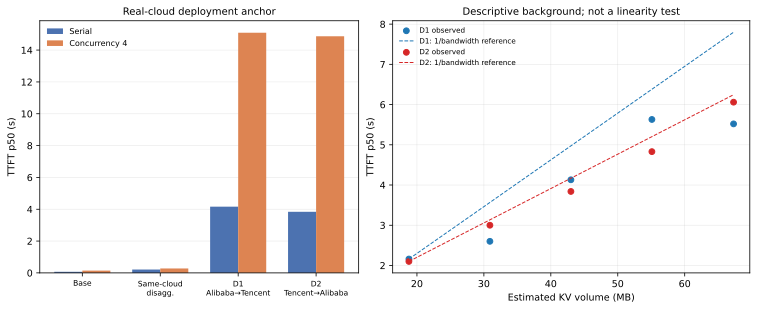
\includegraphics[width=\columnwidth]{figures/fig_cloudttft.svg}
\caption{Real-cloud deployment anchor. (a) Median TTFT for same-cloud and cross-cloud
configurations under serial and four-way concurrency. (b) C-stage TTFT against estimated KV
volume for five fixed prompt groups. Dashed lines are anchored $1/\mathrm{bandwidth}$ engineering
references; this panel is a \emph{descriptive background}, not a linearity test. D-mini was planned
but not executed.}
\label{fig:cloudttft}
\end{figure}
